A ViT-B-16 modell sb-photothemes-imagenet114 adathalmazon teljes tanítással történt tesztelésének eredménye. Lásd a soron következő ábrákat és táblázatokat a mérések eredményeihez.
\subsubsection{ViT-B-16 teljes tanítás folyamata}
\begin{itemize} 
	\item Epoch 1/10 - train: 2259/2259 [16:01<00:00,  2.35it/s]
	\item Epoch 1/10 - val: 282/282 [00:42<00:00,  6.70it/s]
	\item Epoch 1: Train loss=1.2851, acc=0.6443 Val loss=1.1000, acc=0.6794
	\item Epoch 2/10 - train: 2259/2259 [16:00<00:00,  2.35it/s]
	\item Epoch 2/10 - val: 282/282 [00:42<00:00,  6.69it/s]
	\item Epoch 2: Train loss=0.8488, acc=0.7472 Val loss=0.9895, acc=0.7195
	\item Epoch 3/10 - train: 2259/2259 [16:00<00:00,  2.35it/s]
	\item Epoch 3/10 - val: 282/282 [00:42<00:00,  6.68it/s]
	\item Epoch 3: Train loss=0.6250, acc=0.8080 Val loss=0.9986, acc=0.7340
	\item Epoch 4/10 - train: 2259/2259 [16:01<00:00,  2.35it/s]
	\item Epoch 4/10 - val: 282/282 [00:42<00:00,  6.67it/s]
	\item Epoch 4: Train loss=0.4766, acc=0.8511 Val loss=1.0406, acc=0.7300
	\item Epoch 5/10 - train: 2259/2259 [16:01<00:00,  2.35it/s]
	\item Epoch 5/10 - val: 282/282 [00:42<00:00,  6.68it/s]
	\item Epoch 5: Train loss=0.3783, acc=0.8815 Val loss=1.0650, acc=0.7371
	\item Epoch 6/10 - train: 2259/2259 [16:01<00:00,  2.35it/s]
	\item Epoch 6/10 - val: 282/282 [00:42<00:00,  6.67it/s]
	\item Epoch 6: Train loss=0.3202, acc=0.9000 Val loss=1.1107, acc=0.7365
	\item Epoch 7/10 - train: 2259/2259 [16:01<00:00,  2.35it/s]
	\item Epoch 7/10 - val: 282/282 [00:42<00:00,  6.67it/s]
	\item Epoch 7: Train loss=0.2771, acc=0.9137 Val loss=1.1609, acc=0.7377
	\item Epoch 8/10 - train: 2259/2259 [16:01<00:00,  2.35it/s]
	\item Epoch 8/10 - val: 282/282 [00:42<00:00,  6.67it/s]
	\item Epoch 8: Train loss=0.2482, acc=0.9230 Val loss=1.1802, acc=0.7378
	\item Epoch 9/10 - train: 2259/2259 [16:01<00:00,  2.35it/s]
	\item Epoch 9/10 - val: 282/282 [00:42<00:00,  6.67it/s]
	\item Epoch 9: Train loss=0.2237, acc=0.9297 Val loss=1.2074, acc=0.7470
	\item Epoch 10/10 - train: 2259/2259 [16:01<00:00,  2.35it/s]
	\item Epoch 10/10 - val: 282/282 [00:42<00:00,  6.67it/s]
	\item Epoch 10: Train loss=0.2083, acc=0.9355 Val loss=1.2559, acc=0.7426
\end{itemize}

\subsubsection{ViT-B-16 teljes tanítás folyamata}
  \begin{figure}[H]
    \centering
    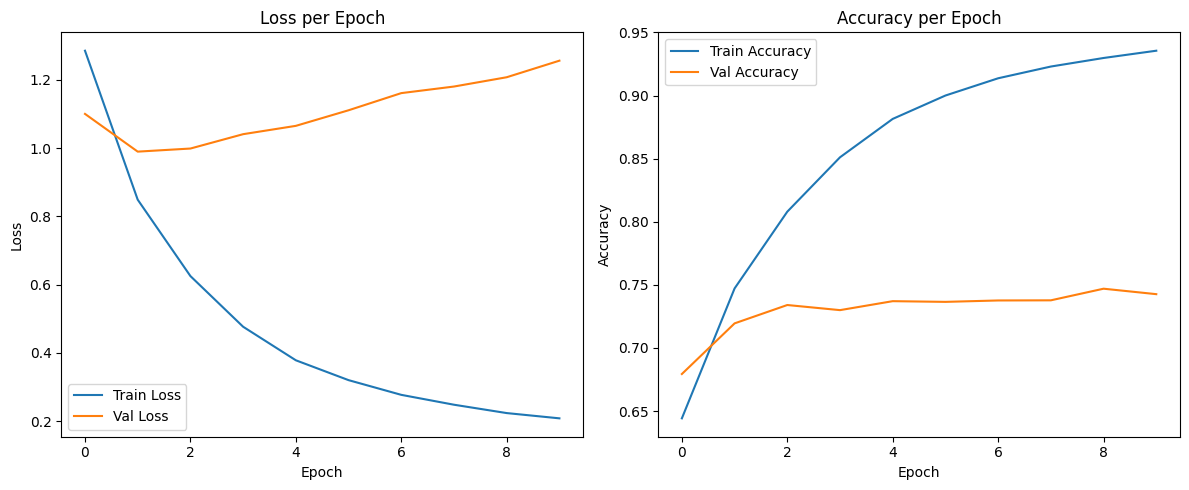
\includegraphics[width=1.0\textwidth]{images/phase02/ViT-B-16_learning_curve.png}
    \caption{ViT-B-16 teljes tanítás utáni sima Confusion Mátrix}
    \label{fig:phase02_ViT-B-16_learning_curves}
  \end{figure}

\subsubsection{ViT-B-16 teljes tanítás utáni eredményei}
  \begin{center}
  \begin{longtable}{l c}
  \caption{ViT-B-16 teljes tanítás utáni vizsgálati eredményei} \label{tab:phase02_ViT-B-16} \\
  \toprule
  \textbf{Metrika} & \textbf{Érték} \\
  \midrule
  \endfirsthead
  \toprule
  \textbf{Metrika} & \textbf{Érték} \\
  \midrule
  \endhead
  Top-1 Accuracy & 0.7414 \\
  Top-5 Accuracy & 0.9257 \\
  Precision & 0.6935 \\
  Recall & 0.6636 \\
  F1-score & 0.6730 \\
  Inference time & 42.40 sec \\
  \bottomrule
  \end{longtable}
  \end{center}

\subsubsection{ViT-B-16 eredményeinek összehasonlítása}
  \begin{center}
  \begin{longtable}{l c c}
  \caption{ViT-B-16 eredményeinek összehasonlítása} \label{tab:phase02_ViT-B-16_compare} \\
  \toprule
  \textbf{Metrika} & \textbf{Pretrained} & \textbf{Fine-tuned} \\
  \midrule
  \endfirsthead
  \toprule
  \textbf{Metrika} & \textbf{Pretrained} & \textbf{Fine-tuned} \\
  \midrule
  \endhead
  Top-1 Accuracy  & 0.5308 & 0.7414 \\
  Top-5 Accuracy & 0.8582 & 0.9257 \\
  Precision & 0.4629 & 0.6935 \\
  Recall & 0.4419 & 0.6636 \\
  F1-score & 0.4307 & 0.6908 \\
  Inference time & 92.13 sec & 42.40 sec \\
  \bottomrule
  \end{longtable}
  \end{center}

\subsubsection{ViT-B-16 eredményeinek összehasonlítása}
  \begin{figure}[H]
    \centering
    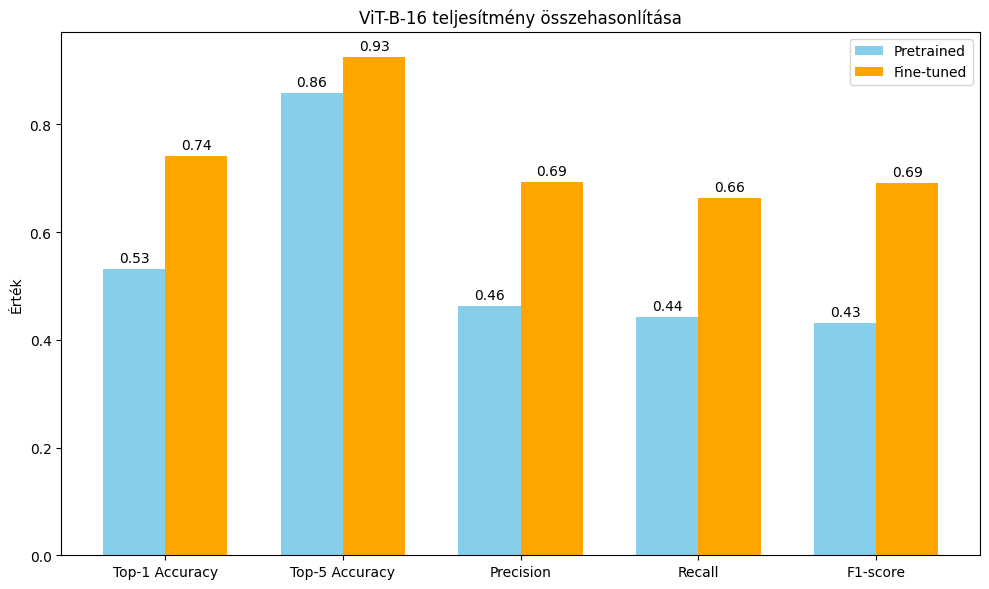
\includegraphics[width=1.0\textwidth]{images/phase02/ViT-B-16_compare01.png}
    \caption{ViT-B-16 eredményeinek összehasonlítása}
    \label{fig:ViT-B-16_compare01}
  \end{figure}

\subsubsection{ViT-B-16 eredményeinek összehasonlítása}
  \begin{figure}[H]
    \centering
    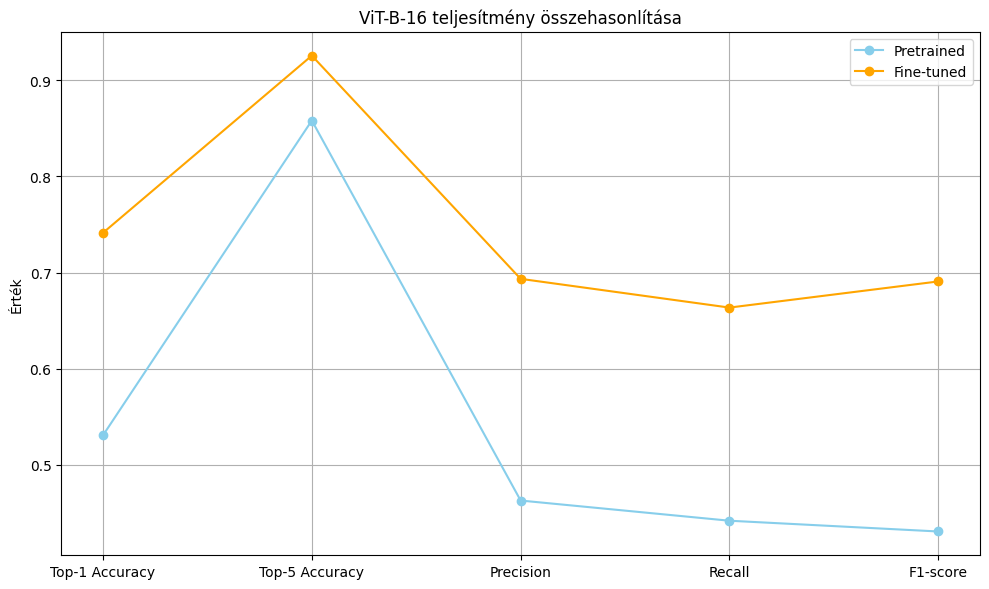
\includegraphics[width=1.0\textwidth]{images/phase02/ViT-B-16_compare02.png}
    \caption{ViT-B-16 eredményeinek összehasonlítása}
    \label{fig:ViT-B-16_compare02}
  \end{figure}

\subsubsection{ViT-B-16 teljes tanítás utáni sima Confusion Mátrix}
  \begin{figure}[H]
    \centering
    
\includegraphics[width=1.0\textwidth]{images/phase02/ViT-B-16_basic_conf_mat.png}
    \caption{ViT-B-16 teljes tanítás utáni sima Confusion Mátrix}
    \label{fig:phase02_ViT-B-16_basic_conf_mat}
  \end{figure}

  \subsubsection{ViT-B-16 Confusion Mátrixok összehasonlítása}
  \begin{figure}[H]
    \centering
    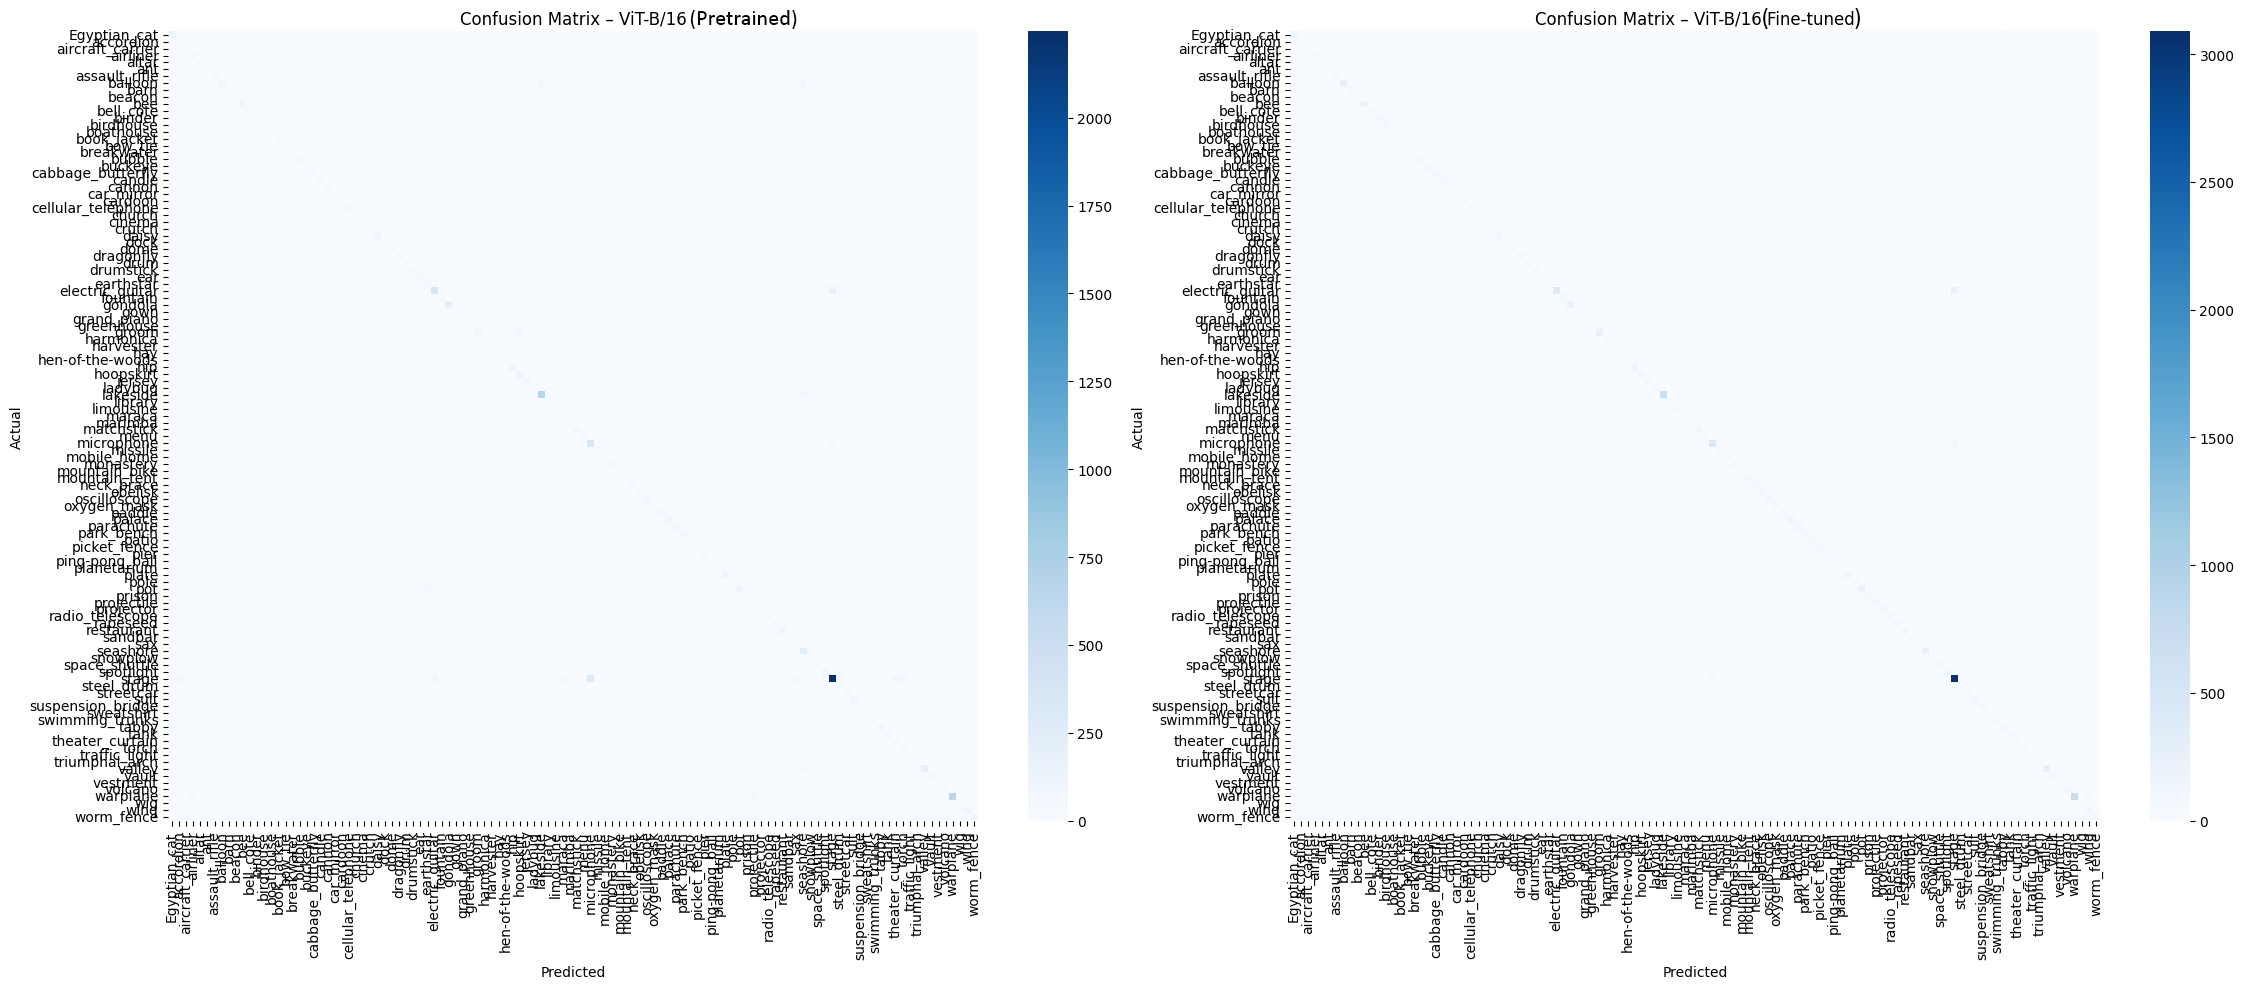
\includegraphics[width=1.0\textwidth]{images/phase02/ViT-B-16_basic_conf_mat_compare.png}
    \caption{ViT-B-16 sima Confusion Mátrixok összehasonlítása}
    \label{fig:phase02_ViT-B-16_basic_conf_mat_compare}
  \end{figure}

  \subsubsection{ViT-B-16 teljes tanítás utáni normalizált Confusion Mátrix}
  \begin{figure}[H]
    \centering
    
\includegraphics[width=1.0\textwidth]{images/phase02/ViT-B-16_normalised_conf_mat.png}
    \caption{ViT-B-16 teljes tanítás utáni normalizált Confusion Mátrix}
    \label{fig:phase02_ViT-B-16_normalised_conf_mat}
  \end{figure}

  \subsubsection{ViT-B-16 normalizált Confusion Mátrixok összehasonlítása}
  \begin{figure}[H]
    \centering
    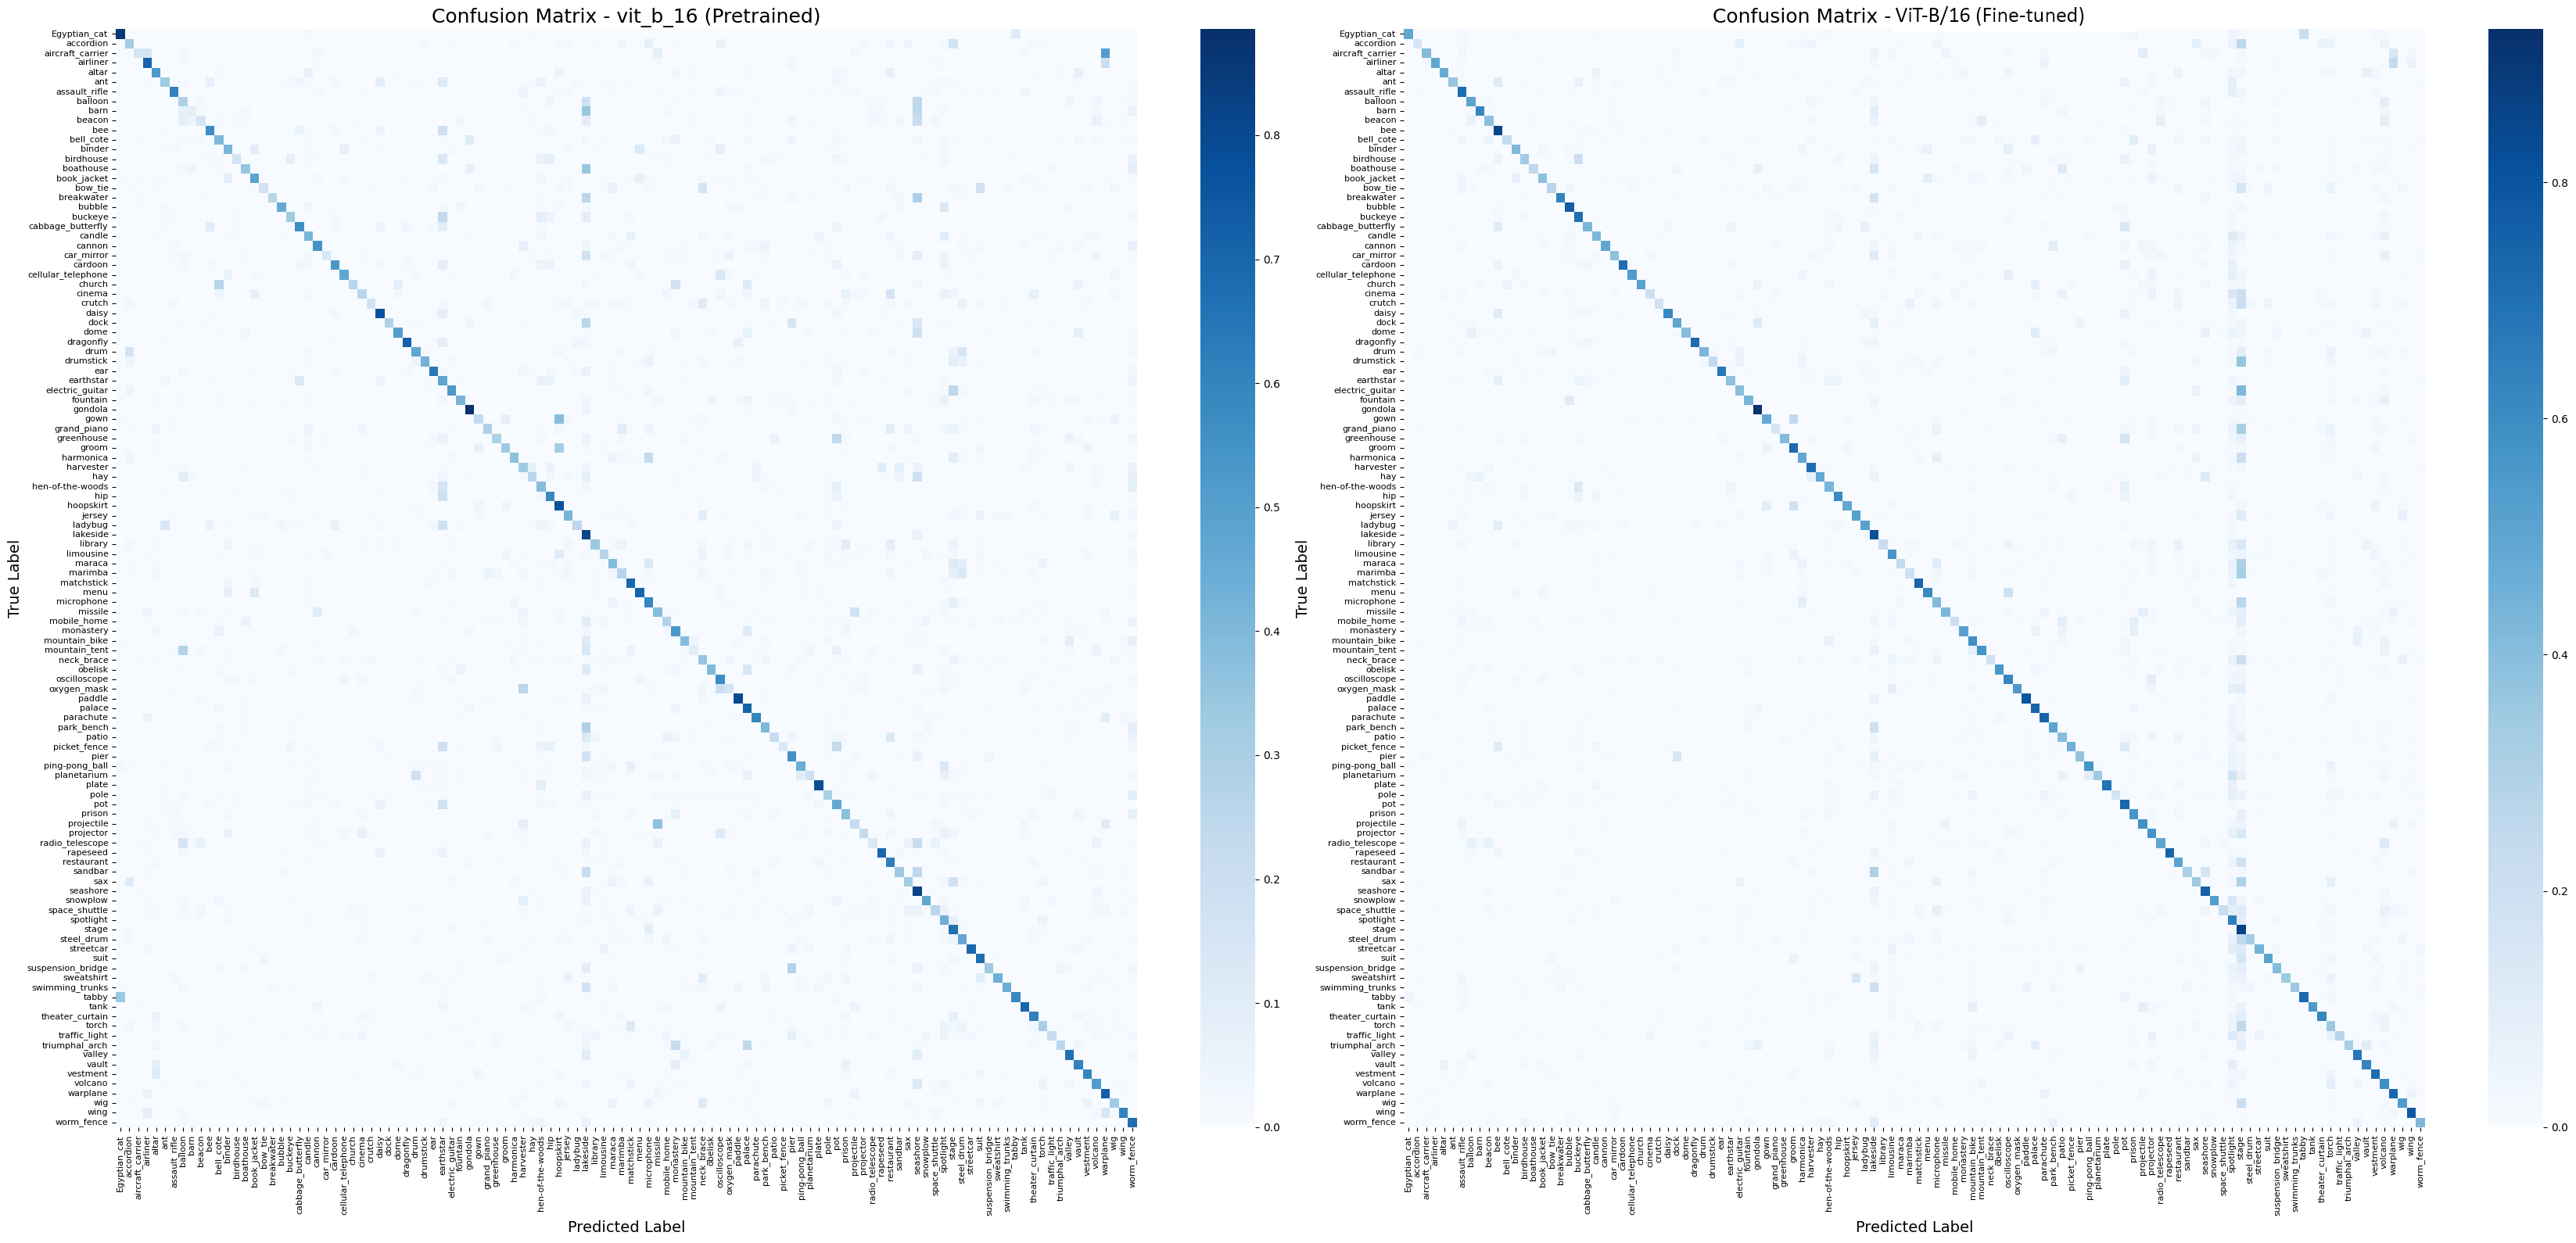
\includegraphics[width=1.0\textwidth]{images/phase02/ViT-B-16_normalised_conf_mat_compare.png}
    \caption{ViT-B-16 normalizált Confusion Mátrixok összehasonlítása}
    \label{fig:phase02_ViT-B-16_normalised_conf_mat_compare}
  \end{figure}

\subsubsection{ViT-B-16 teljes tanítás utáni részletes osztályonkénti metrikák}
  \begin{center}
\begin{longtable}{lllll}
\caption{ViT-B-16 teljes tanítás utáni részletes osztályonkénti metrikák}\label{tab:phase2_ViT-B-16_class_table}\\
\toprule
class & precision & recall & f1-score & support \\
\midrule
\endfirsthead
\toprule
class & precision & recall & f1-score & support \\
\midrule
\endhead
warplane & 0.93 & 0.87 & 0.90 & 871 \\
paddle & 0.92 & 0.84 & 0.88 & 93 \\
rapeseed & 0.91 & 0.79 & 0.85 & 77 \\
plate & 0.89 & 0.89 & 0.89 & 143 \\
gondola & 0.88 & 0.94 & 0.91 & 227 \\
daisy & 0.87 & 0.87 & 0.87 & 149 \\
dragonfly & 0.87 & 0.81 & 0.84 & 75 \\
church & 0.86 & 0.71 & 0.78 & 35 \\
tank & 0.86 & 0.82 & 0.84 & 78 \\
missile & 0.84 & 0.52 & 0.65 & 82 \\
tabby & 0.83 & 0.79 & 0.81 & 107 \\
Egyptian-cat & 0.82 & 0.81 & 0.82 & 145 \\
groom & 0.82 & 0.79 & 0.81 & 285 \\
stage & 0.82 & 0.91 & 0.87 & 3380 \\
bell-cote & 0.81 & 0.55 & 0.65 & 77 \\
ear & 0.81 & 0.74 & 0.77 & 80 \\
electric-guitar & 0.81 & 0.62 & 0.70 & 687 \\
worm-fence & 0.81 & 0.61 & 0.69 & 137 \\
cellular-telephone & 0.80 & 0.78 & 0.79 & 104 \\
hip & 0.80 & 0.78 & 0.79 & 195 \\
oscilloscope & 0.79 & 0.76 & 0.77 & 143 \\
suspension-bridge & 0.79 & 0.70 & 0.74 & 127 \\
valley & 0.79 & 0.86 & 0.82 & 295 \\
bee & 0.78 & 0.83 & 0.81 & 212 \\
hoopskirt & 0.78 & 0.80 & 0.79 & 135 \\
lakeside & 0.78 & 0.87 & 0.82 & 801 \\
bubble & 0.76 & 0.77 & 0.77 & 100 \\
drumstick & 0.76 & 0.56 & 0.64 & 126 \\
matchstick & 0.76 & 0.74 & 0.75 & 127 \\
oxygen-mask & 0.76 & 0.75 & 0.76 & 143 \\
triumphal-arch & 0.76 & 0.75 & 0.75 & 55 \\
airliner & 0.75 & 0.72 & 0.74 & 80 \\
greenhouse & 0.75 & 0.59 & 0.66 & 51 \\
monastery & 0.75 & 0.71 & 0.73 & 112 \\
suit & 0.75 & 0.77 & 0.76 & 141 \\
sweatshirt & 0.75 & 0.54 & 0.63 & 80 \\
swimming-trunks & 0.75 & 0.57 & 0.65 & 79 \\
vestment & 0.75 & 0.77 & 0.76 & 69 \\
aircraft-carrier & 0.74 & 0.51 & 0.61 & 39 \\
dome & 0.74 & 0.75 & 0.75 & 85 \\
jersey & 0.74 & 0.66 & 0.70 & 154 \\
pole & 0.74 & 0.47 & 0.57 & 136 \\
projectile & 0.74 & 0.76 & 0.75 & 117 \\
assault-rifle & 0.73 & 0.82 & 0.77 & 91 \\
balloon & 0.73 & 0.75 & 0.74 & 338 \\
barn & 0.73 & 0.72 & 0.73 & 111 \\
library & 0.73 & 0.55 & 0.63 & 74 \\
picket-fence & 0.73 & 0.62 & 0.67 & 118 \\
restaurant & 0.73 & 0.74 & 0.73 & 141 \\
snowplow & 0.73 & 0.79 & 0.76 & 62 \\
cabbage-butterfly & 0.72 & 0.62 & 0.67 & 101 \\
dock & 0.72 & 0.60 & 0.65 & 84 \\
ladybug & 0.72 & 0.72 & 0.72 & 108 \\
microphone & 0.71 & 0.70 & 0.70 & 596 \\
menu & 0.70 & 0.84 & 0.77 & 68 \\
altar & 0.69 & 0.73 & 0.71 & 59 \\
cardoon & 0.69 & 0.87 & 0.77 & 55 \\
drum & 0.69 & 0.67 & 0.68 & 49 \\
fountain & 0.69 & 0.66 & 0.68 & 92 \\
hay & 0.69 & 0.62 & 0.65 & 73 \\
palace & 0.69 & 0.83 & 0.75 & 139 \\
pot & 0.69 & 0.77 & 0.73 & 254 \\
seashore & 0.69 & 0.83 & 0.76 & 289 \\
theater-curtain & 0.69 & 0.80 & 0.74 & 80 \\
traffic-light & 0.69 & 0.41 & 0.52 & 58 \\
book-jacket & 0.68 & 0.52 & 0.59 & 90 \\
hen-of-the-woods & 0.68 & 0.56 & 0.61 & 105 \\
obelisk & 0.68 & 0.72 & 0.70 & 95 \\
radio-telescope & 0.68 & 0.64 & 0.66 & 108 \\
wing & 0.68 & 0.87 & 0.77 & 148 \\
pier & 0.66 & 0.63 & 0.65 & 97 \\
ping-pong-ball & 0.66 & 0.74 & 0.70 & 91 \\
space-shuttle & 0.66 & 0.50 & 0.57 & 84 \\
streetcar & 0.66 & 0.71 & 0.68 & 65 \\
boathouse & 0.65 & 0.56 & 0.60 & 43 \\
spotlight & 0.65 & 0.50 & 0.57 & 202 \\
steel-drum & 0.65 & 0.56 & 0.60 & 84 \\
candle & 0.64 & 0.62 & 0.63 & 111 \\
neck-brace & 0.64 & 0.46 & 0.54 & 137 \\
cannon & 0.63 & 0.69 & 0.66 & 55 \\
gown & 0.63 & 0.50 & 0.56 & 66 \\
mountain-tent & 0.63 & 0.83 & 0.72 & 121 \\
planetarium & 0.63 & 0.44 & 0.51 & 62 \\
vault & 0.63 & 0.79 & 0.70 & 104 \\
cinema & 0.62 & 0.45 & 0.52 & 51 \\
earthstar & 0.62 & 0.61 & 0.61 & 121 \\
harvester & 0.62 & 0.76 & 0.68 & 71 \\
parachute & 0.62 & 0.83 & 0.71 & 117 \\
ant & 0.61 & 0.46 & 0.53 & 95 \\
bow-tie & 0.61 & 0.52 & 0.56 & 67 \\
grand-piano & 0.61 & 0.48 & 0.54 & 63 \\
limousine & 0.61 & 0.70 & 0.65 & 119 \\
mountain-bike & 0.61 & 0.47 & 0.53 & 66 \\
binder & 0.60 & 0.77 & 0.68 & 105 \\
buckeye & 0.60 & 0.67 & 0.63 & 101 \\
sandbar & 0.60 & 0.59 & 0.59 & 83 \\
volcano & 0.60 & 0.57 & 0.59 & 119 \\
breakwater & 0.59 & 0.69 & 0.63 & 58 \\
mobile-home & 0.59 & 0.52 & 0.55 & 83 \\
projector & 0.59 & 0.66 & 0.62 & 157 \\
birdhouse & 0.58 & 0.57 & 0.58 & 116 \\
park-bench & 0.58 & 0.61 & 0.59 & 144 \\
prison & 0.58 & 0.66 & 0.62 & 101 \\
patio & 0.54 & 0.59 & 0.56 & 144 \\
marimba & 0.53 & 0.35 & 0.42 & 79 \\
wig & 0.53 & 0.54 & 0.54 & 70 \\
torch & 0.51 & 0.48 & 0.50 & 116 \\
crutch & 0.47 & 0.42 & 0.44 & 105 \\
accordion & 0.46 & 0.26 & 0.33 & 47 \\
beacon & 0.45 & 0.55 & 0.49 & 62 \\
car-mirror & 0.42 & 0.49 & 0.45 & 68 \\
harmonica & 0.42 & 0.52 & 0.46 & 100 \\
maraca & 0.42 & 0.28 & 0.34 & 90 \\
sax & 0.38 & 0.41 & 0.39 & 112 \\
\midrule
accuracy &  &  & 0.74 & 18172 \\
macro avg & 0.69 & 0.66 & 0.67 & 18172 \\
weighted avg & 0.74 & 0.74 & 0.74 & 18172 \\
\bottomrule
\end{longtable}
\end{center}


\subsubsection{GPU memóriahasználat}
\begin{itemize}
  \item aktív GPU: NVIDIA A100-SXM4-40GB
  \item GPU memória (lefoglalt): 1.09 GB
  \item GPU memória (használt):  0.29 GB
\end{itemize}

\subsubsection{Legrosszabbul teljesítő osztályok}
  \begin{center}
    \begin{longtable}{llll}
    \caption{Legrosszabbul teljesítő osztályok}\label{tab:phase02_ViT-B-16_legrosszabb_osztlyok}\\
    \toprule
    Class & Precision & Recall & F1-score \\
    \midrule
    \endfirsthead
    \toprule
    Class & Precision & Recall & F1-score \\
    \midrule
    \endhead
    sax & 0.38 & 0.41 & 0.39 \\
    harmonica & 0.42 & 0.52 & 0.46 \\
    car-mirror & 0.42 & 0.49 & 0.45 \\
    maraca & 0.42 & 0.28 & 0.34 \\
    beacon & 0.45 & 0.55 & 0.49 \\
    accordion & 0.46 & 0.26 & 0.33 \\
    crutch & 0.47 & 0.42 & 0.44 \\
    torch & 0.51 & 0.48 & 0.50 \\
    marimba & 0.53 & 0.35 & 0.42 \\
    planetarium & 0.63 & 0.44 & 0.51 \\
    \bottomrule
    \end{longtable}
  \end{center}